\chapter{Opis projektnog zadatka}
		
		\par Društvene mreže za vlasnike ljubimaca nisu zaživjele u svijetu, a tradicionalnim društvenim mrežama nedostaju značajke koje puno znače vlasnicima. Ideja je da "Naši Ljubimci" bude točka okupljanja, komunikacije i razmjene iskustva između vlasnika kućnih ljubimaca i tvrtki.
		\par Ciljana skupina zainteresirana za rješenje su vlasnici kućnih ljubimaca poput mački i pasa, ali i oni s egzotičnijim ljubimcima. Osim njih, velik je interes tvrtki koje žele vlasnicima približiti svoje proizvode i usluge koje pružaju u domeni kućnih ljubimaca.
		\par BarkHappy je mobilna aplikacija za vlasnike pasa s ciljem povezivanja i stvaranja zajednice vlasnika pasa. Bazirana je na lokaciji vlasnika i sadrži slične funkcionalnosti kao projektni zadatak, s najvećom razlikom što je ekskluzivna za vlasnike pasa, a ne za sve kućne ljubimce.
		
		\begin{figure}[H]
			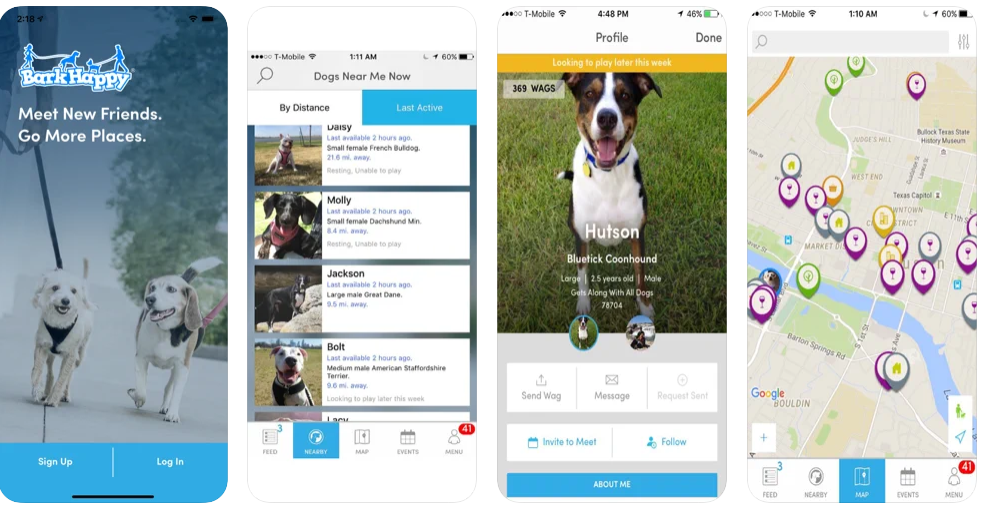
\includegraphics[scale=0.4]{slike/BarkHappy.PNG} %veličina slike u odnosu na originalnu datoteku i pozicija slike
			\centering
			\caption{BarkHappy}
			\label{fig:promjene}
		\end{figure}
	
		\par Yummypets je web i mobilna aplikacija za vlasnike kućnih ljubimaca svih vrsta, s naglaskom na dijeljenje fotografija i videa u stilu Instagrama. Aplikacija je vrlo sličnih funkcionalnosti kao projektni zadatak, a najveće razlike su postojanje dediciranog foruma i funkcije pronalaska najbliže veterinarske postaje.
		
		\begin{figure}[H]
			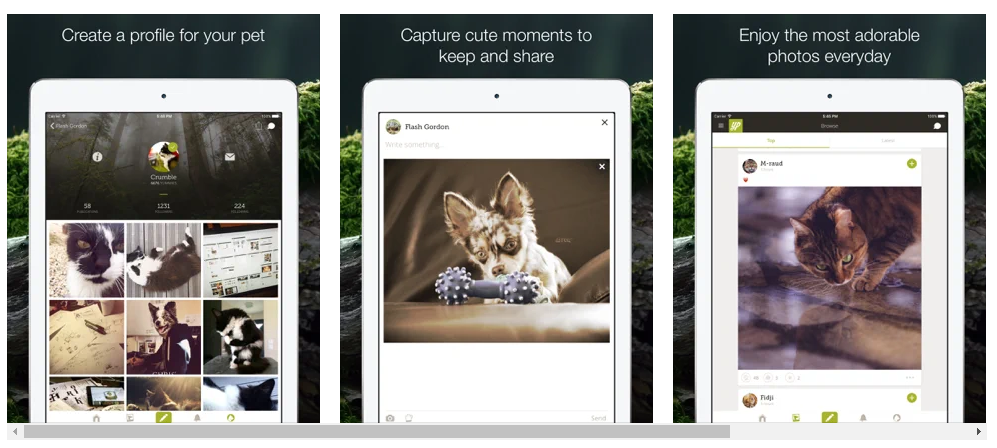
\includegraphics[scale=0.4]{slike/Yummypets.PNG} %veličina slike u odnosu na originalnu datoteku i pozicija slike
			\centering
			\caption{Yummypets}
			\label{fig:promjene}
		\end{figure}
	
		\par Cilj projektnog zadatka je aplikacija "Naši Ljubimci". Zamišljena je kao društvena mreža za vlasnike kućnih ljubimaca i tvrtke koje pružaju usluge vezane uz skrb o ljubimcima. Za korištenje aplikacije nužna je registracija korisnika. Potrebni osobni podaci su:
		
		
		\begin{packed_item}
			\item ime
			\item prezime
			\item adresa e-pošte
			\item željeno korisničko ime
		\end{packed_item}
		
		\par Tijekom registracije, korisnik mora odabrati jednu od željenih kategorija: vlasnik ljubimca ili tvrtka (obrt). 
		\par \underbar{Vlasnik ljubimca} može uređivati vlastiti profil, što podrazumjeva promjenu profilne fotografije, promjenu adrese e-pošte te stvaranje profila svojih ljubimaca. Svaki ljubimac unutar vlasnikovog profila ima svoj zaseban profil. Kategorije kućnih ljubimaca su sljedeće:
		
		\begin{packed_item}
			\item psi
			\item mačke
			\item mali glodavci
			\item ptice
			\item gmazovi
			\item egzotično 
		\end{packed_item}
	
		\par Za pojedinog ljubimca potrebno je unijeti ime, dob, spol, profilnu fotografiju i kratki opis. Za pse i mačke potrebno je dodatno evidentirati pasmina, a za sve ostale kategorije potrebno je evidentirati točnu vrstu životinje. Sve profile ljubimaca je moguće naknadno uređivati (promjena osnovnih podataka te profilne fotografije) te je moguće objavljivati fotografije i video uratke o ljubimcu uz kratak opis objave. U sklopu medijske galerije, vlasnici na svom profilu mogu objavljivati foto i video materijale s kratkim opisom (poput zajedničkih fotografija s jednim ili više ljubimaca). Vlasnici mogu poslati zahtjev za prijateljstvom drugim vlasnicima, koji ga onda mogu prihvatiti, odbiti ili trajno blokirati. Prijatelji međusobno vide medijske galerije te mogu ostavljati kratke komentare. Vlasnik profila ima pravo brisanja neželjenih komentara te prekida prijateljstva. Aplikacija podržava kreiranje događaja (evenata). Svaki vlasnik može stvoriti novi događaj, kojim će ostale vlasnike potenicijalno potaknuti na druženje. Svaki novi događaj mora sadržavati:
		
		\begin{packed_item}
			\item datum
			\item trajanje
			\item lokaciju 
			\item opis
		\end{packed_item}
		Dogovaranje sastanaka unutar Naši Ljubimci, bit će povezano s Google Calendar sustavom zbog lakše potvrde dolaska (RVSP). Vlasnik događaj može dijeliti samo s prijateljima ili sa svim registriranim korisnicima. Svi korisnici kojima je događaj vidljiv imaju opciju odabira statusa dolaska: 
		\begin{packed_item}
			\item "dolazim"
			\item "možda"
			\item "ne dolazim" 
		\end{packed_item}
		Također je moguće ostaviti kratki komentar na događaj.
		
		\par \underbar{Tvrtka (obrt)} na svom profilu prijavljuje jednu ili više od dostupnih usluga:
		\begin{packed_item}
			\item čuvanje
			\item odgoj
			\item briga o zdravlju 
		\end{packed_item}
		Podaci o tvrki (naziv, adresa, kontakt) na njenom profilu vidljivi su svim registriranim korisnicima, uz detaljan opis ponuđenih usluga. Tvrtke na svom profilu mogu objavljivati foto i video materijale te kratke poruke na koje svi korisnici mogu odgovarati. Tvrtke također mogu stvarati nove događaje, na koje se mogu prijaviti svi korisnici aplikacije.
		
		\par Svi korisnici aplikacije mogu pretraživati druge korisnike te si međusobno slati direktne poruke. U slučaju zlouporabe aplikacije, svi korisnici mogu prijaviti drugog korisnika ili tvrtku administratoru.
		
		\par \underbar {Administratori} aplikacije nemaju javne profile, niti se tretiraju kao vlasnici ljubimaca. Oni imaju mogućnost blokiranja ili trajnog brisanja profila korisnika, ukoliko se za to pojavi potreba.
		
		\par Ovaj sustav ima velikog potencijala za proširenje i nadogradnju. Evo nekoliko ideja za budućnost:
		\begin{packed_item}
			\item \textit {end-to-end} enkripcija direktnih poruka za veću privatnost
			\item 2-faktorska autentikacija za bolju sigurnost
			\item predlaganje novih prijatelja na temelju geolokacije
			\item dodavanje \textit {feeda} s novim objavama korisnikovih prijatelja
			\item dodavanje mogućnosti plaćenih oglasa u vidu istaknutih objava za tvrtke i obrte
		\end{packed_item}
		
		
		\eject
		
		
	